\section{Offline evaluation}
\begin{itemize}
	\item Evaluating an IR system without any interaction with user 
	\item Assumption: assessors can tell what is relevant
\end{itemize}
\subsection{Collection-based evaluation}
\begin{itemize}
	\item Approximating user happiness by relevance of the found documents
	\item There are different measures to do that
\end{itemize}
\subsubsection{Traditional Evaluation measures}
\begin{itemize}
	\item We can view IR as a (binary) classification problem where every document is either relevant or not with respect to a query
	\item The evaluation is performed by calculating precision ($\frac{TP}{TP+FP}$) and recall ($\frac{TP}{TP+FN}$)
	\item However, the output of an IR system is a ranking and not a binary classification. Thus, we label the first $k$ documents the system proposes as relevant, and other as non-relevant $\implies$ precision/recall $@$ cut-off ($P@k$/$R@k$)
	\item The trade-off between precision and recall is task specific. For web searches, we want a high precision on the first few documents, but allow a worse recall (as a user doesn't want to find \textit{all} relevant documents). In contrast, in medicine, we want to have a high recall to not miss an important document
	\item Another way to incorporate precision and recall for ranking is using R/P curves. We start with a cut-off point of 0 where precision is 1 and recall 0. Then we increase the cut-off point one by one and record the new values in the curve (left, Figure~\ref{img:offline_eval_RP_curves}). While the cut-off rank heads to infinity, recall goes to 1 and precision to 0. We interpolate the curves by taking the maximum value of all future values/values right from a given point.
	\begin{figure}[ht]
		\centering
		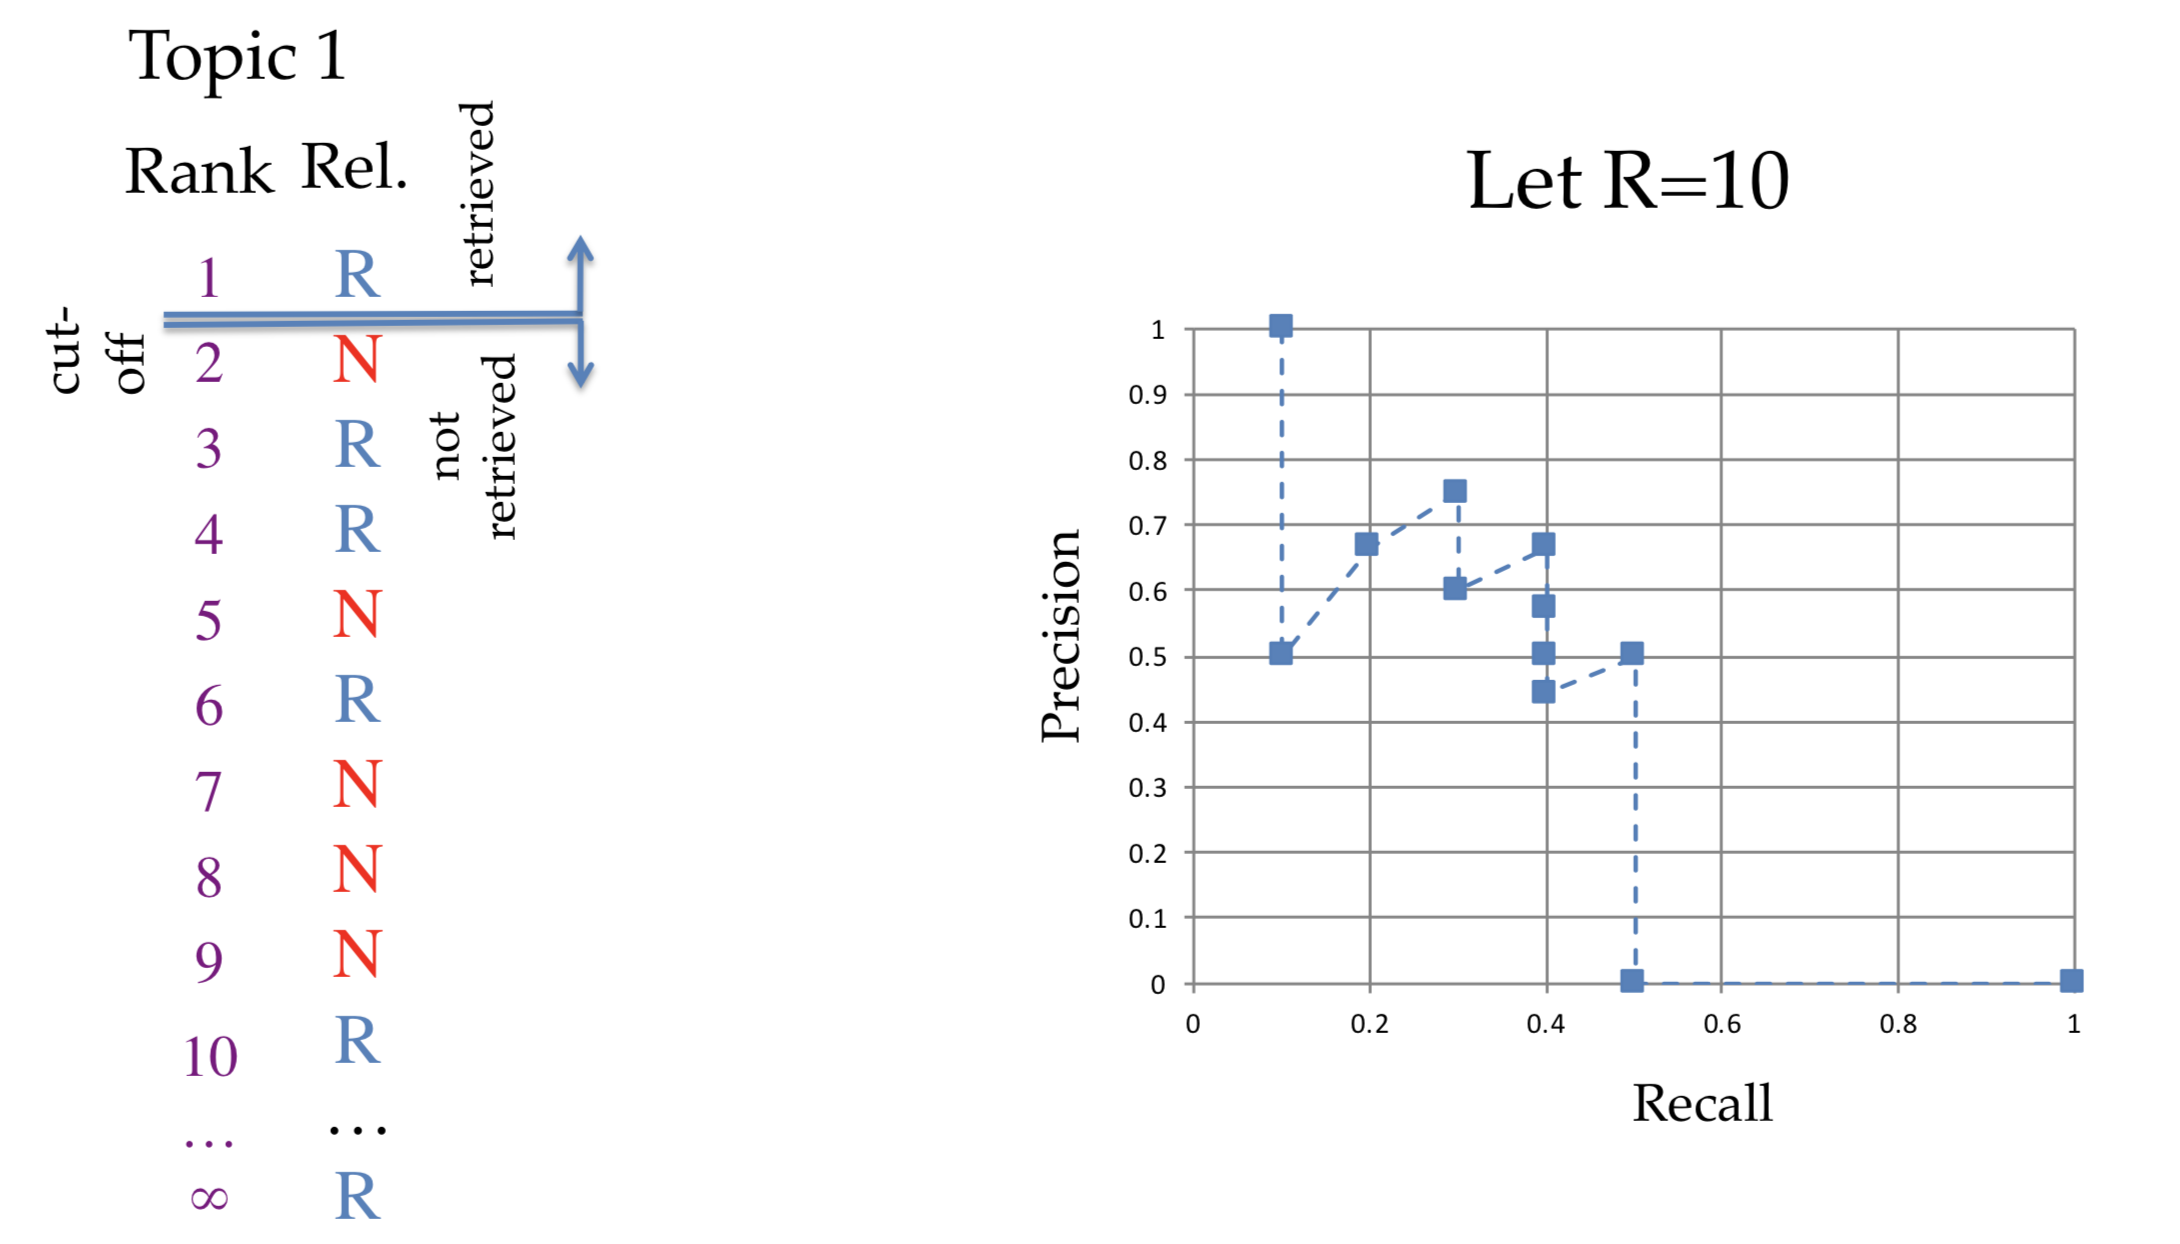
\includegraphics[width=0.4\textwidth]{figures/offline_eval_RP_curves.png}
		\caption{R/P curves for ranking}
		\label{img:offline_eval_RP_curves}
	\end{figure}
	\item When having multiple queries, we would average the RP curves. 
	\item The area under the curve is the average precision which can also be calculated by taking the average of all precision values at ranks with relevant documents.
	\item Usually, a binary scale of whether a document is relevant is not sufficient. For a graded relevance scale, we can use different evaluation measures
	\begin{itemize}
		\item \textbf{Discounted Cumulative Gain (DCG)} - considers the relevance grade and position of every document. The total gain is accumulated at a certain rank $k$:
		$$DCG@k = \sum\limits_{\text{rank} r=1}^{k} \frac{2^{\text{rel}_r} - 1}{\log_2\left(1 + r\right)}$$
		\item The numerator is the non-linear relevance score of the document at rank $r$, and the denominator the discount over ranking position
		\item The score highly depends on the best possible ranking for a query. Thus, the DCG can be normalized by the value of the best ranking $\implies$ $0\leq nDCG \leq 1$. This makes it easier to compare scores over different queries
	\end{itemize}
\end{itemize}
\subsubsection{Model-based Evaluation measures}
\begin{itemize}
	\item Another perspective of evaluation is looking at different aspects of possibles metrics. A model-based approach considers the following three components:
	\begin{enumerate}
		\item \textbf{Browsing model} - describes how the user interacts with results, like the probability of a document being clicked/viewed $\Rightarrow p(d)$
		\item \textbf{Model of document utility} - describes how a user derives utility from individual relevant documents. Similar to how to determine the graded relevance scale $\Rightarrow g(d)$.
		\item \textbf{Utility accumulation model} - describes how a user accumulates utility in the course of browsing $\Rightarrow E\left[g(D)\right] = \sum_{r=1}^{\infty}g(d) \cdot p(d)$
	\end{enumerate}
	\item Examples for the browsing models
	\begin{itemize}
		\item \textit{Position-based models} - the chance of observing a document depends on the position in the ranking. We can for example model it by $\Rightarrow p(d_r)=(1-\theta)^{r-1} \theta$. The corresponding utility accumulation is described by Rank-biased Precision (RBP): $RBP = \sum_{r=1}^{\infty}\text{rel}_r (1-\theta)^{r-1} \theta$
		\item \textit{Cascade-based models} - considers $\theta$ as a function of the document at rank $r$. Mostly, the following function is used: $\theta_r = \mathcal{R}(\text{rel}_r) = \frac{2^{\text{rel}_r}-1}{2^{\text{max rel}}}$. The corresponding utility accumulation is the \textit{Expected Reciprocal Relevance}: $ERR@k = \sum\limits_{r=1}^{k} \frac{1}{r} \cdot \theta_r \cdot \prod\limits_{i=1}^{r-1}\left(1 - \theta_i\right)$
	\end{itemize}
\end{itemize}
\subsubsection{Collection construction}
\begin{itemize}
	\item To evaluate a system offline, we need labels of whether a document is relevant with respect to a query (or graded scale) $\Rightarrow$ labels are created by humans
	\item First step is to generate a huge document collection, and generate a set of topics/queries that should be evaluated. Mostly, queries are selected from very frequent, common and rare query bin sets of highly-used search engines 
	\item To be able to calculate measures like recall, we need to find all relevant documents in the collection. Can be done either deterministically or stochastically
	\begin{itemize}
		\item \textbf{Depth-k pooling} - deterministic, standard method. Apply $M$ IR systems and take the union of the $k$ top results of all $M$ systems. This set of documents is labeled by humans, and all others are considered as not relevant. Note that we need the $M$ systems to be different/take another perspective on the data so that they don't find all the same documents. Otherwise, future IR algorithms can find relevant documents that the others haven't found yet and will be punished for that. $k$ is task specific, but a value of $100$ has shown to be sufficient
		\item \textbf{Random Sampling} - stochastic method. Simplest approach is for a query $q$, just sample a small set of documents out of the whole corpus and label those. Otherwise are considered as unlabeled, thus neglected in evaluation. Problem: significant sparsity of relevant documents in the corpus. 
	\end{itemize}
\end{itemize}
\subsection{Challenges of offline evaluation}
\label{sec:offline_eval_problems}
\begin{itemize}
	\item Expensive and slow to collect new data
	\item Ambiguous queries are particularly hard to judge realistically (what intent is most popular?). Particularly hard for personalized searches
	\item Judges need to correctly appreciate uncertainty/allow different intents
	\item How to identify when relevance changes (temporal, query intent changes, ...)?
\end{itemize}
\subsection{Comparative evaluation}
\begin{itemize}
	\item How do we compare different retrieval systems? Is the difference only due to random noise? $\implies$ Statistical significance test
	\item Two hypotheses where we want to prove that $H_0$ is wrong: $$H_0: \text{MAP}_E - \text{MAP}_P = 0, \hspace{4mm} H_1: \underbrace{\text{MAP}_E - \text{MAP}_P \neq 0}_{\text{two-sided}} \text{\hspace{2mm}or\hspace{2mm}}\underbrace{\text{MAP}_E - \text{MAP}_P > 0}_{\text{one-sided}}$$
	\item Compute the $p$-value that describes the probability of observing the test data given that $H_0$ is valid (low $p$-value disprove null hypothesis)
\end{itemize}
\subsubsection{Student's t-test}
\begin{itemize}
	\item Statistic: $$t=\frac{\mu_{E-P}}{\frac{\sigma_{E-P}}{\sqrt{N}}} = \frac{\overline{AP_E - AP_P}}{\frac{\sigma_{E-P}}{\sqrt{N}}}$$
	\item We assume that the mean measure follow a normal distribution (see Figure~\ref{img:hypothesis_testing_t_test_t_dist})
	\begin{figure}[ht]
		\centering
		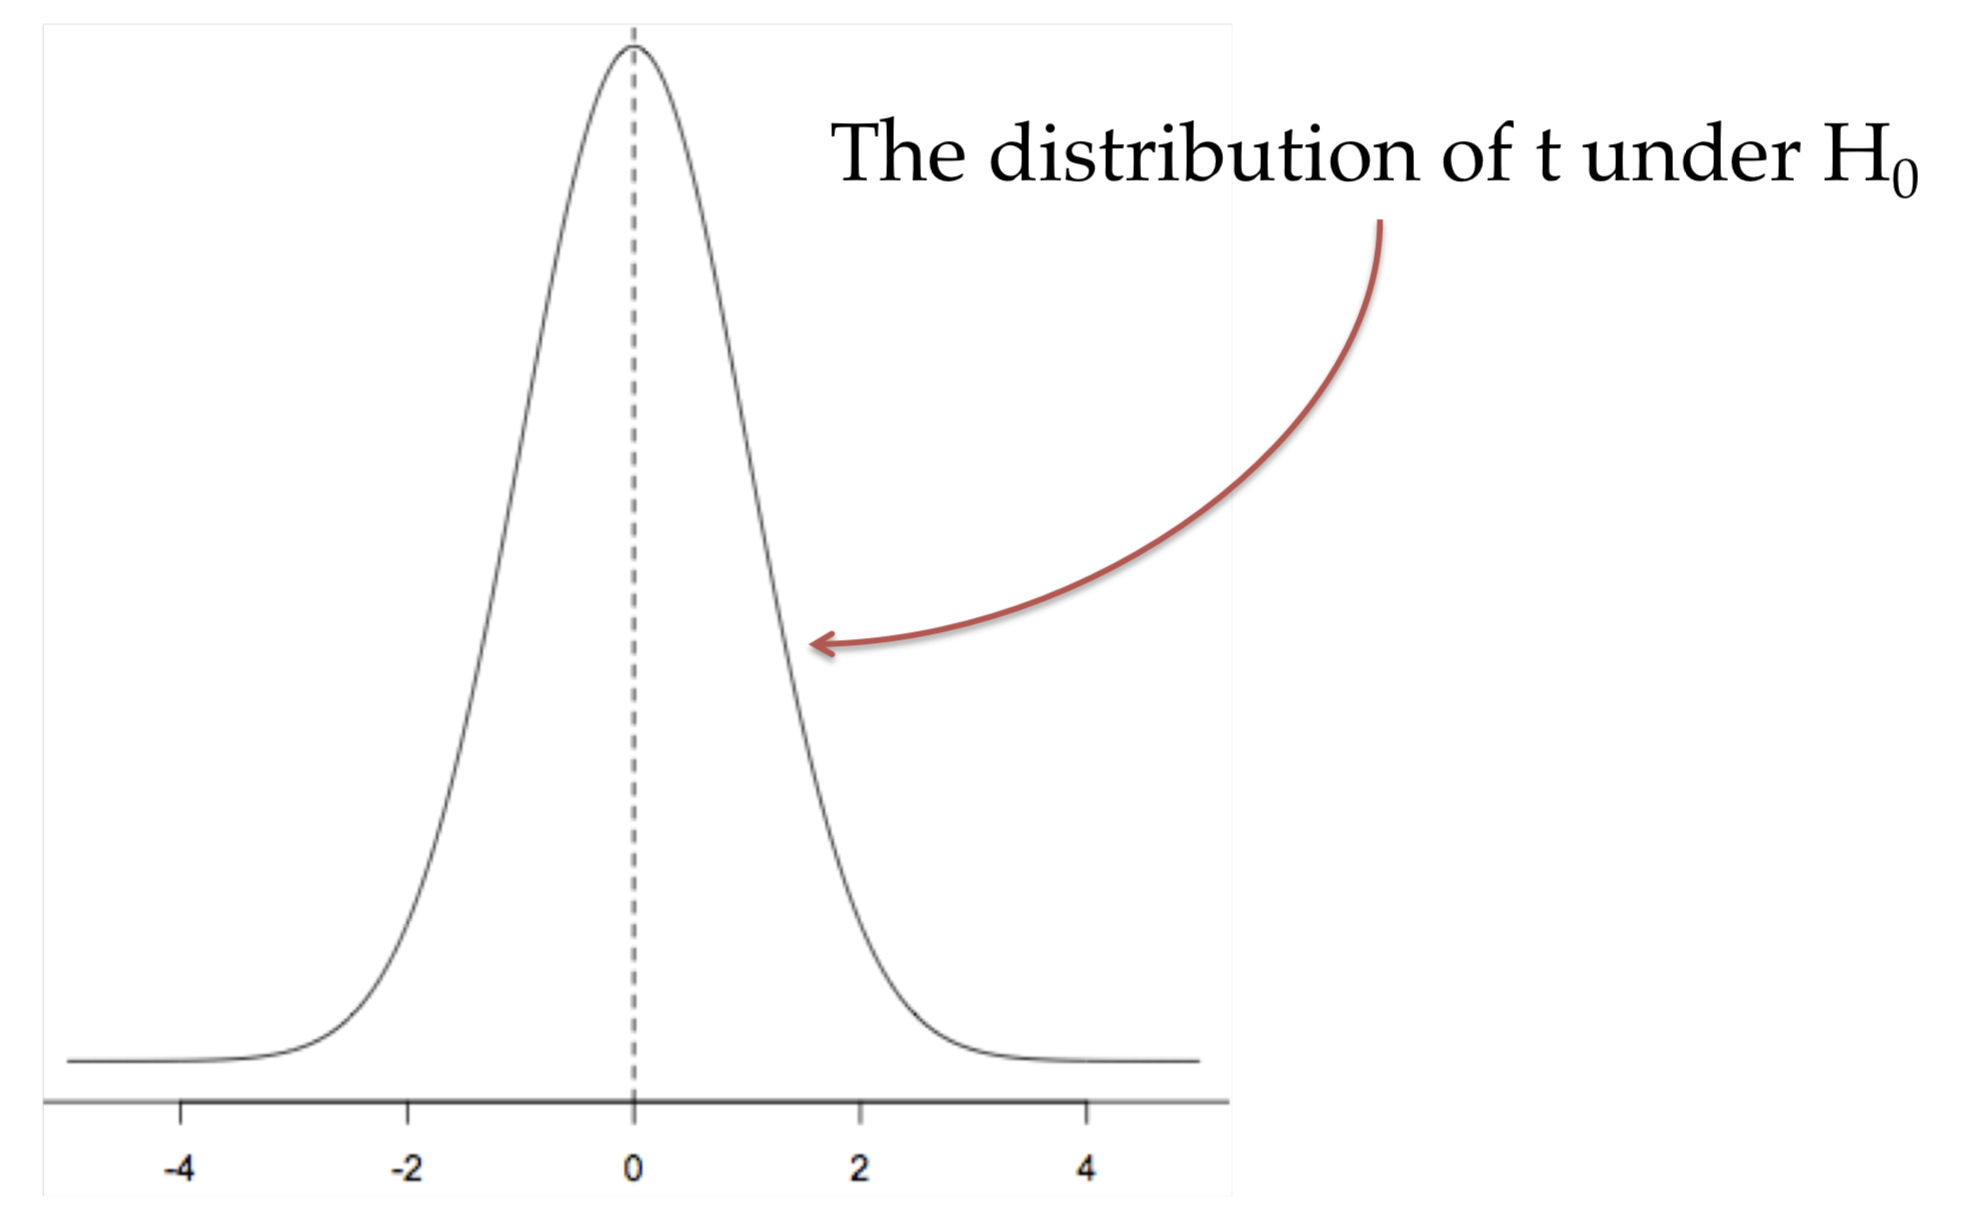
\includegraphics[width=0.3\textwidth]{figures/hypothesis_testing_t_test_t_dist.png}
		\caption{Distribution of $t$ values under the null hypothesis}
		\label{img:hypothesis_testing_t_test_t_dist}
	\end{figure}
	\item The $p$-value is determined by the area under the distribution right from the determined value
	\item If the $p$-value is lower than the significance level $\alpha$, reject null hypothesis
	\item There are two different error types for the t-test: 
	\begin{description}
		\item[Type 1] rejecting null hypothesis although it was true (prob. is $\alpha$)
		\item[Type 2] not rejecting the null hypothesis although it was false (prob. is $\beta$)
	\end{description}
	\item There are four aspects of the test that interact with each other. If one is unknown, it can be derived from the others
	\begin{enumerate}
		\item \textit{Sample size} $N$
		\item \textit{Effect size} = diff. of means / std. dev.
		\item \textit{Significance level} = Type 1 error $\alpha$
		\item \textit{Power} = 1 - Type 2 error $\beta$. Prob. of finding an effect if it is there. 
	\end{enumerate}
\end{itemize}
\subsubsection{Sign test}
\begin{itemize}
	\item Look at score/sample pairs from $A$ and $B$ and consider the null hypothesis $H_0: P(B>A)=P(A>B)=1/2$.
	\item It is a discrete way of looking at the t-test. For a sample size of $N$, we get a binomial distribution with $N$ bins. The bins summed up from the measured number of $B$ winning over $A$ describe the p-value (see Figure~\ref{img:hypothesis_testing_sign_test})
	\begin{figure}[ht]
		\centering
		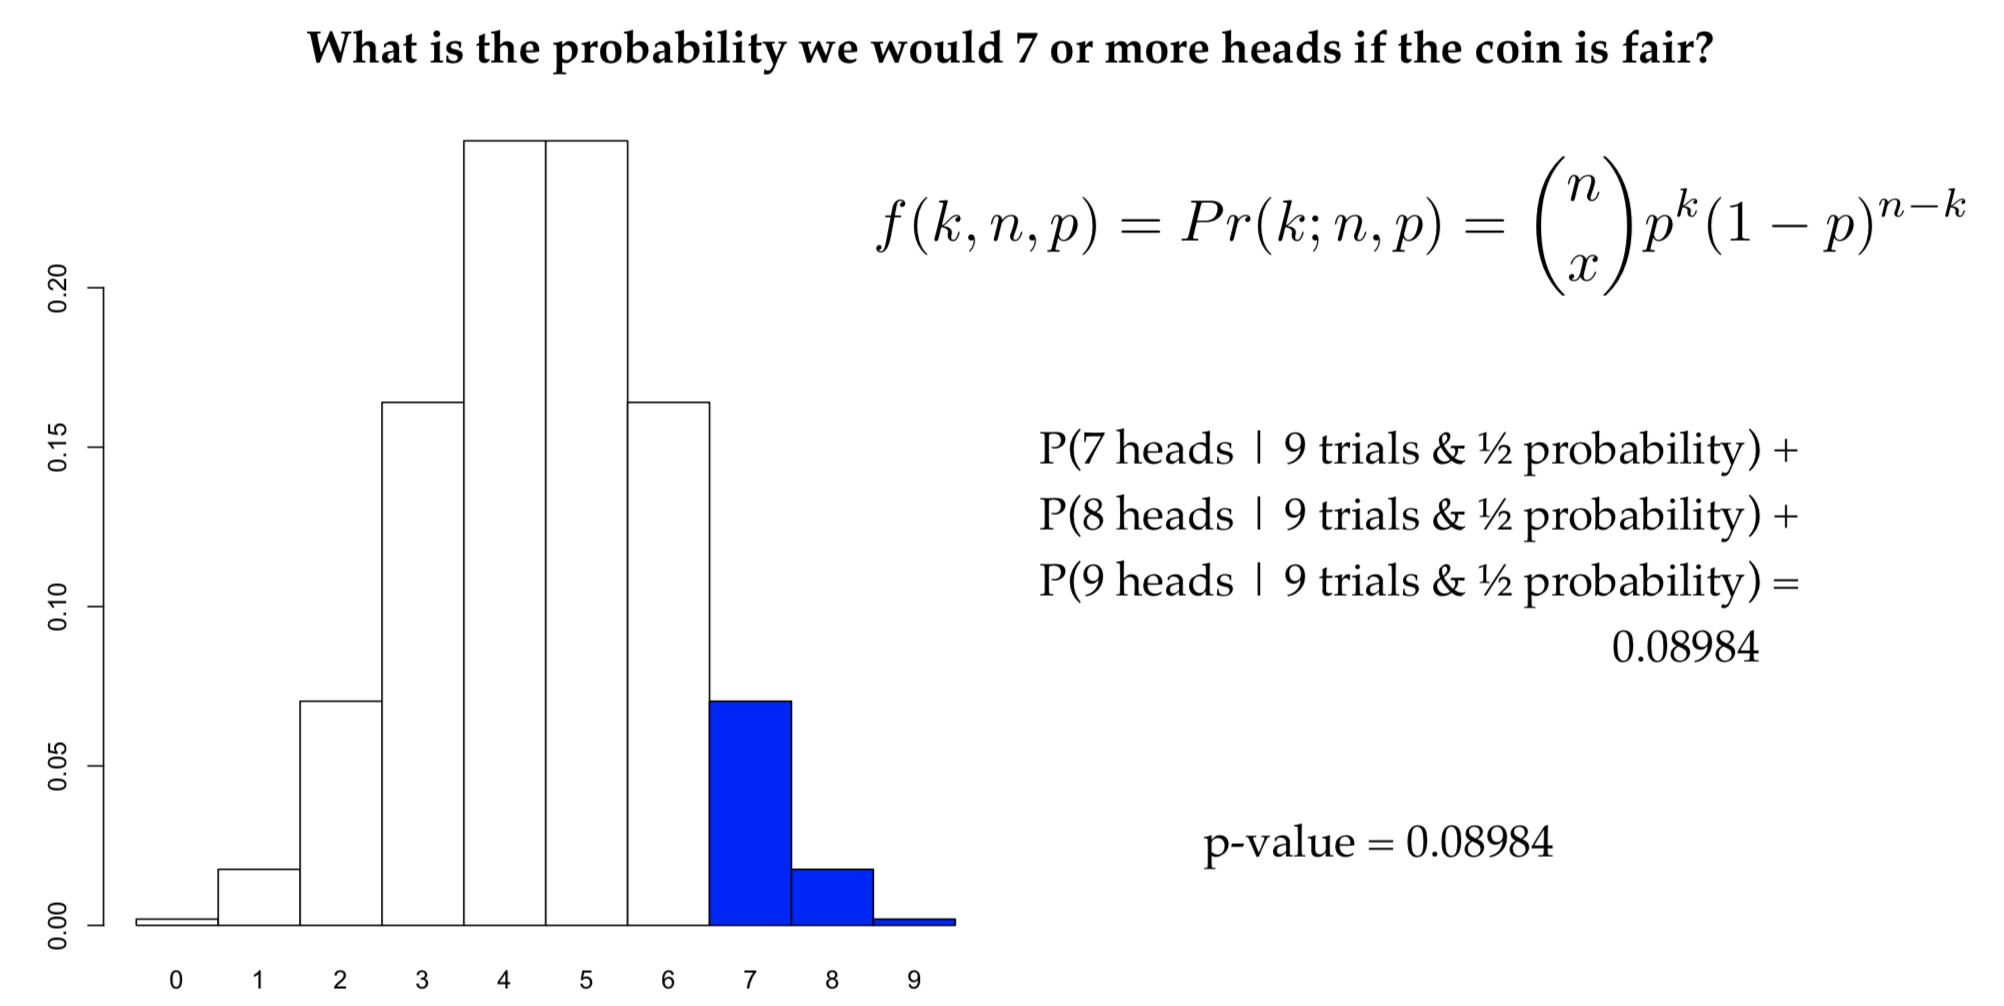
\includegraphics[width=0.4\textwidth]{figures/hypothesis_testing_sign_test.png}
		\caption{Distribution of $t$ values under the null hypothesis}
		\label{img:hypothesis_testing_sign_test}
	\end{figure}
\end{itemize}
\subsubsection{Distribution-free tests}
\begin{itemize}
	\item Tests where we do not explicitly assume the underlying data to be sampled from a specific distribution
	\item \textbf{Randomization test}
	\begin{itemize}
		\item Given: a set of results for $N$ queries for algorithm $A$ and $B$
		\item Repeat for many times:
		\begin{itemize}
			\item Randomly swap values for a query in algorithm $A$ and $B$
			\item Compute average of both systems and their difference
			\item Add difference to an array
		\end{itemize} 
		\item The two systems are significantly different, if the actual difference without swapping is outside 95\% of the differences in the array.
	\end{itemize}
	\item \textbf{Bootstrap test}
	\begin{itemize}
		\item Same preparation as for randomization test
		\item Repeat for many times:
		\begin{itemize}
			\item Randomly sample pair of scores (i.e. selecting queries) of $A$ and $B$ with replacement
			\item Compute average of each systems in the set of pairs
			\item Add difference to an array
		\end{itemize}
		\item The two systems are significantly different if the mean of the array can be shown to be significantly different from 0.
	\end{itemize}
	
\end{itemize}